
\documentclass{article}
\usepackage{ctex}
\usepackage{amsmath}
\usepackage{graphicx}

\title{期权定价实验}
\author{}
\date{February 2023}

\begin{document}

\maketitle


\vspace{2ex}

\section{变量代换}

我们首先进行变量代换,令$\tau = t-T$,$x = \ln S$,则原方程可以变为:

$$\frac{\partial u}{\partial \tau} + \frac{1}{2}\sigma^2\frac{\partial^2 u}{\partial x^2} + (r-\frac{1}{2}\sigma^2)\frac{\partial u}{\partial x} - r u = 0$$

边界条件变为:$u(x=0, \tau) = 0$,$u(x=x_{\max}, \tau) = e^{x_{\max}}-K$。

终止条件变为:$u(x,\tau=0) = g(x) = \max(x-K,0)$。


\section{构建网格}
我们在计算区域 $[0, x] × [-T, 0]$ 上划分标准网格,记空间方向上步长 $h = \Delta x = \frac{S}{(N + 1)}$,时间方向上步长 $\tau = \Delta t = \frac{T}{M}$。在空间方向上我们已知两个边界的值,而时间方向仅有一个边界条件,因此空间方向比时间方向多离散一个网格,保证最终要求解的网格点数为 $M × N$。

此外,我们使用记号$u_{i,j} \approx u(x_i, t_j) = u(i\Delta x, j\Delta t) = u(ih, j\tau)$,作为数值逼近的解。其中 $i = 0,..., N + 1$,$j = 0,..., M$。需要计算的网格点为 $i = 1,..., N$,$j = 1,..., M$。

% \begin{figure}[h]
%   \centering
%   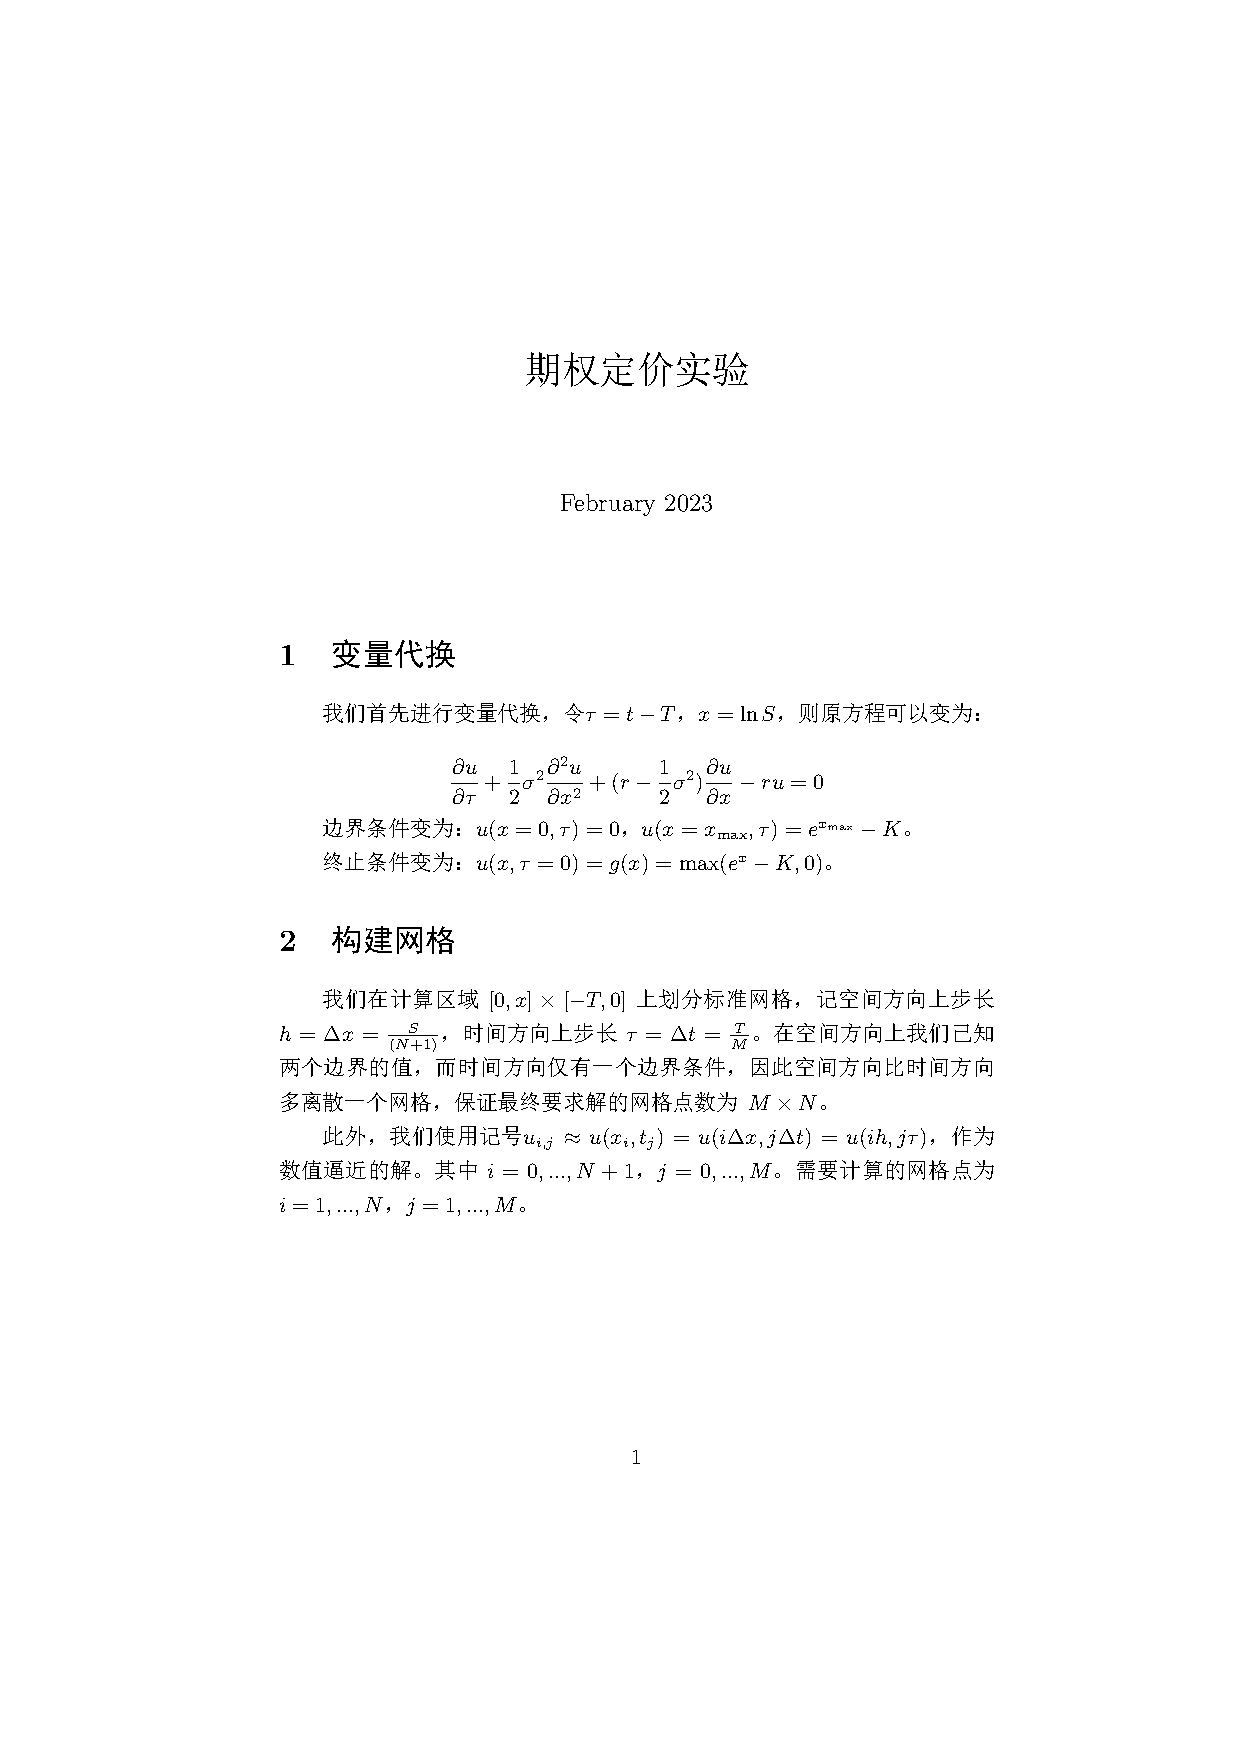
\includegraphics[width=0.5\textwidth]{C:/test.jpg}
%   \caption{这是图片的标题}
%   \label{fig:example}
% \end{figure} 

% 如图 \ref{fig:example} 所示,这是一张图片。



\section{离散方式}


\subsection{空间方向上的离散}

空间方向采用二阶精度的中心差分
$$\frac{\partial u}{\partial x}(x_i, t_j) = \frac{u_{i+1, j} - u_{i-1, j}}{2h}$$
和
$$\frac{\partial^2 u}{\partial x^2}(x_i, t_j) = \frac{u_{i+1, j} - 2u_{i, j} + u_{i-1, j}}{h^2}$$
作为 Black-Scholes 偏微分方程在空间方向上导数的近似。这样就得到半离散方程
$$\frac{\partial u}{\partial \tau} + (\frac{1}{2}\sigma^2)\frac{u_{i+1, j} - 2u_{i, j} + u_{i-1, j}}{h^2} + (r - \frac{1}{2}\sigma^2)\frac{u_{i+1, j} - u_{i-1, j}}{2h} - ru_{i, j} = 0$$
即$$\frac{\partial u}{\partial \tau} + (\frac{h+2}{4h^2}\sigma^2 - \frac{r}{2h})u_{i-1, j} - (r + \frac{\sigma^2}{h^2})u_{i, j} + (\frac{2-h}{4h^2}\sigma^2 + \frac{r}{2h})u_{i+1, j} = 0$$
为了表示方便,我们令
\begin{equation}
\left\{
        \begin{array}{lr}
        \vspace{1ex}
        a = \frac{h+2}{4h^2}\sigma^2 - \frac{r}{2h}, & \\
        \vspace{1ex}
        b = - (r + \frac{\sigma^2}{h^2}), & \\
        \vspace{1ex}
        c = \frac{2-h}{4h^2}\sigma^2 + \frac{r}{2h}. &  
        \end{array}
\right.
\nonumber
\end{equation}

记$\bar{u_j} = (u_{1, j}, u_{2, j},...,u_{N, j})^T$,当指标$i$取遍$1,2,...,N$时,得到半离散方程组
$$\frac{\partial u}{\partial \tau} + B\bar{u_j} + z = 0, $$
其中$$B = 
\begin{pmatrix}
    b &   c    &        &        &   & \\
    a &   b    &   c    &        &   & \\
      & \ddots & \ddots & \ddots &   & \\
      &        & \ddots & \ddots & c & \\
      &        &        &   a    & b & \\
\end{pmatrix},
\bar{u_j} = 
\begin{pmatrix}
    u_{1, j}   \\
    u_{2, j}   \\
    \vdots     \\
    u_{N-1, j} \\
    u_{N, j}   \\
\end{pmatrix},
z = 
\begin{pmatrix}
    au_{0, j}   \\
    0           \\
    \vdots      \\
    0           \\
    cu_{N+1, j} \\
\end{pmatrix},
$$


\subsection{空间方向上的离散}

下面我们讨论半离散方程在时间方向上的离散。

我们考虑显式欧拉格式,隐式欧拉格式和 Crank-Nicolson 格式。

\end{document}

